\documentclass{ctexbeamer}        % 文档类beamer的汉化版本

\usefonttheme{serif}              % 使用衬线字体
\usefonttheme{professionalfonts}  % 数学公式字体
\usepackage{amsmath}
\usepackage{mathtools}
\usepackage{hyperref}
\usepackage{listings}
\usepackage{fontspec} % 定制字体
\usepackage{xcolor} % 定制颜色
\usepackage{hyperref}
\definecolor{mygreen}{rgb}{0,0.6,0}
\definecolor{mygray}{rgb}{0.5,0.5,0.5}
\definecolor{mymauve}{rgb}{0.58,0,0.82}
\lstset{ %
backgroundcolor=\color{white},      % choose the background color
basicstyle=\footnotesize\ttfamily,  % size of fonts used for the code
columns=fullflexible,
tabsize=4,
breaklines=true,               % automatic line breaking only at whitespace
captionpos=b,                  % sets the caption-position to bottom
commentstyle=\color{mygreen},  % comment style
escapeinside={\%*}{*)},        % if you want to add LaTeX within your code
keywordstyle=\color{blue},     % keyword style
stringstyle=\color{mymauve}\ttfamily,  % string literal style
frame=none,
rulesepcolor=\color{red!20!green!20!blue!20},
% identifierstyle=\color{red},
language=c++,
}

%% --> 主题和色彩风格
\usetheme{Frankfurt}       %主题和色彩可以自由搭配
\usecolortheme{orchid}     %主题和色彩的样式可参见网页 https://mpetroff.net/files/beamer-theme-matrix/

\newcommand{\qbinom}[2]{\genfrac{[}{]}{0pt}{}{#1}{#2}}
\newcommand{\stirling}[2]{\genfrac\{ \} {0pt}{}{#1}{#2}}
\newcommand{\lcm}{\operatorname{lcm}}

\begin{document}

%% --> 导言页
%
\title{整除性}
\author{Quack}
\date{\today}
\frame{\titlepage}

%% --> 目录结构
%
\begin{frame}{目录}         %自动生成目录
  \tableofcontents[hideallsubsections]
\end{frame}

%% --> 正式内容开始
%
\section{带余除法和整除}    % 第 1 节

%% 每一节开头显示目录,并高亮当前节的主题
\AtBeginSection[]{\frame{\tableofcontents[currentsection,hideallsubsections]}}

%% --> 第 1 帧
\begin{frame}{带余除法和整除}

\begin{definition}[带余除法]
    设$a,b$为两个正整数,定义带余除法$a / b$:商为正整数$k$,余数为正整数$r$,满足$a=kb+r$且$0 \le r < b$。

    商$k$记为$\lfloor \frac{a}{b} \rfloor$,余数$r$记为$a \bmod b$。
\end{definition}

\begin{example}
    $5$除以$3$的带余除法,商为$1$,余数为$2$。

    余数的一个常见应用是进制转换。
\end{example}

\end{frame}

%% --> 第 2 帧
\begin{frame}{带余除法和整除}

\begin{definition}[整除]
    若$a \bmod b = 0$,则称$a$是$b$的倍数,$b$是$a$的因数(因子),$a$被$b$整除,$b$整除$a$,记为$b|a$。
\end{definition}

\begin{example}
    $9$除以$3$的带余除法,余数为$0$,所以$3|9$。
\end{example}

\end{frame}

\section{公因数}

\begin{frame}{公因数}

\begin{definition}[公因数和公倍数]
    我们把多个数共有的因数和倍数叫做这些数的公因数和公倍数。

    这些数的公因数中,最大的公因数叫做最大公因数(gcd),最小的公倍数叫做最小公倍数(lcm)。
\end{definition}

\begin{example}
    $30$是$2$的倍数,也是$3$的倍数,所以,$30$是$2,3$的公倍数。$2,3$的最小公倍数是$6$,一般写成$\lcm(2,3)=[2,3]=6$。

    $4$是$24$的因数,也是$8$的因数,所以,$4$是$24,8$的公因数。$24,8$的最小公因数是$8$,一般写成$\gcd(24,8)=(24,8)=8$。
\end{example}

\end{frame}

\begin{frame}{公因数}

\begin{definition}[互质]
    若两个数的最大公因数为$1$,则称这两个数互质。
\end{definition}

\begin{example}
    因为$\gcd(8,15)=1$,所以$8$和$15$互质。
\end{example}

\end{frame}

\begin{frame}{公因数}
如何求两个数的gcd?下面的定理给了保证:

\begin{theorem}[辗转相除法]
    $$\gcd(a,b)=\gcd(b,a \bmod b)$$
\end{theorem}
\pause
\begin{proof}
    设$u$同时整除$a$和$b$,则存在$s,t$,使得$a=su,b=tu$。

    令$r = a \bmod b, k = \lfloor \frac{a}{b} \rfloor$,则$a=kb+r$。

    把$a=su,b=tu$代入,得到$su=ktu+r$,即$r=(s-kt)u$,得到$u$也整除$r$。

    反过来,对每一个同时整除$b$和$r$的数$v$,也能得到$v$整除$a$。

    综上,$a$和$b$的每一个公因子也是$b$和$r$的公因子;反过来,$b$和$r$的每一个公因子也是$a$和$b$的公因子。所以,$a$和$b$的所有公因子集合就和$b$和$r$的所有公因子集合相同,所以$\gcd(a,b)=\gcd(b,r)$。
\end{proof}

\end{frame}

\begin{frame}[fragile]
\frametitle{公因数}

根据上述定理,不难写出求两个数gcd的代码:
\begin{block}{辗转相除法}
\begin{lstlisting}[language={c++},
                   numbers=left]
int gcd(int a, int b){return b?gcd(b,a%b):a;}
\end{lstlisting}
\end{block}
由于每两次递归后($(a,b)\rightarrow(b,a \bmod b)\rightarrow(a\bmod b,b \bmod(a\bmod b))$),两个参数都缩小至少一半,所以时间复杂度为$O(\log n)$,其中$n=\min(a,b)$。
\end{frame}

\begin{frame}[fragile]
\frametitle{公因数}

根据上述定理,不难写出求两个数gcd的另一个版本的代码:
\begin{block}{Binary GCD algorithm}
\begin{lstlisting}[language={c++},
                   numbers=left]
int gcd(int a, int b){
    if (a == b) return a;
    if ((a & 1) && (b & 1)) return gcd(b, abs(a - b));
    else if ((a & 1) && (!(b & 1))) return gcd(a, b >> 1);
    else if ((!(a & 1)) && (b & 1)) return gcd(a >> 1, b);
    else return gcd(a >> 1, b >> 1) << 1;
}
\end{lstlisting}
\end{block}
不难发现时间复杂度也为$O(\log n)$,其中$n=\max(a,b)$。

这种方法的好处是避免取模,写高精度gcd的时候可以考虑。
\end{frame}

\section{裴蜀定理}

\begin{frame}{裴蜀定理}

\begin{theorem}[裴蜀定理]
    对于任意正整数$a,b$,存在整数$s,t$,使得$sa+tb=\gcd(a,b)$。
\end{theorem}

\begin{definition}[扩展欧几里得算法]
   对于给定的正整数$a,b$, 扩展欧几里得(exgcd)算法能求出一组$s,t$,使得$sa+tb=\gcd(a,b)$。
\end{definition}

\begin{proof}
    证明的思路是反向模拟辗转相除法从$a,b$求出$\gcd(a,b)$的过程。
\end{proof}

\end{frame}

\begin{frame}{裴蜀定理}

\begin{proof}
    设$r_i$表示辗转相除法的过程中的参数(余数),$r_0=a,r_1=b$。由辗转相除法的过程,有
    $r_n = r_{n-2} \bmod r_{n-1}$。

    由带余除法的定义,设$q_{n-1}$是$r_{n-2}$和$r_{n-1}$做带余除法的商,我们可以改写成
    $r_n = r_{n-2} - r_{n-1}q_{n-1}$。

    设辗转相除法做了$n-1$步停止,则$r_n=\gcd(a,b)$。

    又因为$r_{n-1} = r_{n-3} - r_{n-2}q_{n-2}$,所以有
    \begin{align*}
        &\gcd(a,b)=r_n=r_{n-2} - r_{n-1}q_{n-1}\\
        =&r_{n-2} - (r_{n-3} - r_{n-2}q_{n-2})q_{n-1}\\
        =&(1+q_{n-1}q_{n-2})r_{n-2}-q_{n-1}r_{n-3}
    \end{align*}

    以此类推,最终可以得到$\gcd(a,b)=sr_0+tr_1=sa+tb$。
\end{proof}

\end{frame}

\begin{frame}{裴蜀定理}

\begin{theorem}[裴蜀定理]
    对于任意正整数$a,b$,存在整数$s,t$,使得$sa+tb=\gcd(a,b)$。
\end{theorem}

关于此证明有两点需要注意:

\begin{itemize}
    \item 这只是一种构造$s,t$的方法,只为了证明存在性,实际上满足条件的$s,t$可能不唯一
    \item 由这个证明我们可以设计出递推版本的exgcd算法
\end{itemize}

\end{frame}

\begin{frame}[fragile]
\frametitle{裴蜀定理}
具体来说,有
\begin{align*}
    \gcd(a,b)&=\begin{pmatrix} 0 & 1 \end{pmatrix} \begin{pmatrix} r_{n-1} \\ r_n \end{pmatrix} \\
    &=\begin{pmatrix} 0 & 1 \end{pmatrix} \begin{pmatrix} 0 & 1 \\ 1 & -q_{n-1} \end{pmatrix} \begin{pmatrix} r_{n-2} \\ r_{n-1} \end{pmatrix}\\
    &=\begin{pmatrix} 0 & 1 \end{pmatrix} \begin{pmatrix} 0 & 1 \\ 1 & -q_{n-1} \end{pmatrix} \cdots \begin{pmatrix} 0 & 1 \\ 1 & -q_1 \end{pmatrix} \begin{pmatrix} r_0 \\ r_1 \end{pmatrix}\\
    &=\begin{pmatrix} s & t \end{pmatrix} \begin{pmatrix} r_0 \\ r_1 \end{pmatrix}
\end{align*}
那么我们首先对$a,b$使用辗转相除法,在过程中把$r$数组和$q$数组存下来。
然后根据上述式子递推即可得到一组$s,t$。
\end{frame}

\begin{frame}[fragile]
\frametitle{裴蜀定理}

根据上述算法描述,不难写出递推版exgcd的代码:
\begin{block}{递推版exgcd}
\begin{lstlisting}[language={c++},
                   numbers=left]
void exgcd(int a, int b){
    r[0] = a, r[1] = b;
    int i = 2;
    for ( ; r[i - 1]; i++) {
        r[i] = r[i - 2] % r[i - 1];
        q[i - 1] = r[i - 2] / r[i - 1];
    }
    d = r[i -= 2];
    mat res(1, 0, 0, 1);
    for (int j = i - 1; j; --j)
        res.mul(mat(0, 1, 1, -q[j]));
    s = res.get(1, 0); t = res.get(1, 1);
}
\end{lstlisting}
\end{block}
显然复杂度为$O(\log n)$,其中$n=\min(a,b)$。
\end{frame}

\begin{frame}{裴蜀定理}

不过实际应用中更常见的是递归版本。我们暂时忘记递推版本。

现在我们要求$ax+by=\gcd(a,b)$的整数解,由裴蜀定理我们知道这个方程是存在解的。此外,根据之前辗转相除法的证明过程,$\gcd(a,b)=\gcd(b,a \bmod b)$,所以方程$bx'+(a \bmod b)y'=\gcd(a,b)$也是存在整数解的。

同时,$a \bmod b = a - \lfloor \frac{a}{b} \rfloor b$,所以我们有

$$ax+by=bx'+(a - \lfloor \frac{a}{b} \rfloor b)y'$$

按$a,b$稍作整理,得到

$$ax+by=ay'+b(x'- \lfloor \frac{a}{b} \rfloor y')$$

\end{frame}

\begin{frame}{裴蜀定理}

假如说我们已知方程$bx'+(a \bmod b)y'=\gcd(a,b)$的整数解$x',y'$,那么我们就可以构造出方程$ax+by=\gcd(a,b)$的整数解$x=y',y=x'- \lfloor \frac{a}{b} \rfloor y'$。

只要按照前面计算最大公因数的方法,在递归的过程中加入$x$和$y$的计算就好了。当递归到末尾的时候$b=0$,这时方程有整数解$x=1,y=0$。

\end{frame}

\begin{frame}[fragile]
\frametitle{裴蜀定理}

根据上述算法描述,不难写出递归版exgcd的代码:
\begin{block}{递归版exgcd}
\begin{lstlisting}[language={c++},
                   numbers=left]
int exgcd(int a, int b, int &x, int &y){
    if (!b) {
        x = 1, y = 0;
        return a;
    }
    int d = exgcd(b, a%b, x, y);
    int t = x;
    x = y;
    y = t - a / b * y;
    return d;
}
\end{lstlisting}
\end{block}
显然复杂度为$O(\log n)$,其中$n=\min(a,b)$。
\end{frame}

\begin{frame}{裴蜀定理}

\begin{theorem}[裴蜀定理]
    对于任意正整数$a,b$,存在整数$s,t$,使得$sa+tb=\gcd(a,b)$。
\end{theorem}

由裴蜀定理和gcd的定义能得到一些gcd的性质,如:

\begin{itemize}
    \item $\gcd(ad,bd)=d\gcd(a,b)$
    \item $\gcd(\frac{a}{\gcd(a,b)},\frac{b}{\gcd(a,b)})=1$
    \item 若$c|a,c|b$,则$c|gcd(a,b)$
    \item 若$\gcd(a,b)=1$,则$\gcd(a,bc)=\gcd(a,c)$
\end{itemize}

\end{frame}

\begin{frame}{裴蜀定理}

前三个好证,我们证一下第四个。

\begin{proof}
    证明的思路是证$\gcd(a,bc)|\gcd(a,c)$和$\gcd(a,c)|\gcd(a,bc)$。

    由于$\gcd(a,bc)|a$,所以$\gcd(a,bc)|ac$。并且$\gcd(a,bc)|bc$。所以$\gcd(a,bc)|\gcd(ac,bc)$,即$\gcd(a,bc)|c$。又因为$\gcd(a,bc)|a$,所以$\gcd(a,bc)|\gcd(a,c)$。

    由于$\gcd(a,c)|c$,所以$\gcd(a,c)|bc$,并且$\gcd(a,c)|a$,所以$\gcd(a,c)|\gcd(a,bc)$。
\end{proof}

\end{frame}

\begin{frame}{裴蜀定理}

\begin{theorem}[裴蜀定理]
    对于任意正整数$a,b$,存在整数$s,t$,使得$sa+tb=\gcd(a,b)$。
\end{theorem}

由裴蜀定理也能分析二元一次不定方程$ax+by=c$解的结构。

\begin{itemize}
    \item 对方程$ax+by=c$,方程有解当且仅当$\gcd(a,b)|c$,此时可以用exgcd算法得到方程$ax+by=c$的一组特解$x=x_0,y=y_0$。
    \item 由特解可以得到方程其他的解:$x=x_0+\frac{b}{\gcd(a,b)} \cdot t,y=y_0-\frac{a}{\gcd(a,b)} \cdot t$,其中,$t$为任意整数。
\end{itemize}

\end{frame}

\begin{frame}{裴蜀定理}

\begin{theorem}
    设方程$ax+by=c$的特解为$x=x_0,y=y_0$,那么$x=x_0+\frac{b}{\gcd(a,b)} \cdot t,y=y_0-\frac{a}{\gcd(a,b)} \cdot t$($t$为任意整数)构成了方程所有的解。
\end{theorem}

\begin{proof}
    首先不难验证$x=x_0+\frac{b}{\gcd(a,b)} \cdot t,y=y_0-\frac{a}{\gcd(a,b)} \cdot t$确实是方程的解。
\end{proof}

\end{frame}

\begin{frame}{裴蜀定理}

\begin{proof}
    设$x,y$是方程的任一组解,则有$ax+by=c$,与$ax_0+by_0=c$相减得
    $$a(x-x_0)=b(y_0-y)$$
    从而
    $$\frac{a}{\gcd(a,b)}(x-x_0)=\frac{b}{\gcd(a,b)}(y_0-y)$$
    因为$\gcd(\frac{a}{\gcd(a,b)},\frac{b}{\gcd(a,b)})=1$,所以$\frac{a}{\gcd(a,b)}|y_0-y$。故存在整数$t$,使得$y_0-y=\frac{a}{\gcd(a,b)}t$,即$y=y_0-\frac{a}{\gcd(a,b)}t$。同理有$x=x_0+\frac{b}{\gcd(a,b)}t$。
    
    由$x,y$的任意性,方程的全部解都可以表示为这个形式。
\end{proof}

\end{frame}

\begin{frame}{裴蜀定理}

\begin{theorem}
    设方程$ax+by=c$的特解为$x=x_0,y=y_0$,那么$x=x_0+\frac{b}{\gcd(a,b)} \cdot t,y=y_0-\frac{a}{\gcd(a,b)} \cdot t$($t$为任意整数)构成了方程所有的解。
\end{theorem}

考虑通解在实际问题中的应用:

\begin{itemize}
    \item 如何求所有解中,$x>0$且$x$最小的解?
    \item 如何求在限制$0\le x,y \le C$下,方程的解数?
    \item 如何求所有解中,$|x|+|y|$最小的解?
\end{itemize}

\end{frame}

\begin{frame}{裴蜀定理}

\begin{example}
    如何求所有解中,$x>0$且$x$最小的解$x_{min}$?
\end{example}

由于$x=x_0+\frac{b}{\gcd(a,b)} \cdot t$,所以我们用exgcd先求出$x_0$,设$pr=\frac{b}{\gcd(a,b)}$,那么$x_{min}=(x_0 \bmod pr + pr) \bmod pr$。根据$x_{min}$不难得到其对应的$y$。

\end{frame}

\begin{frame}{裴蜀定理}

\begin{example}
    如何求在限制$0\le x,y \le C$下,方程的解数?
\end{example}

用通解列不等式:

$$0 \le x_0+\frac{b}{\gcd(a,b)} \cdot t < C$$
$$0 \le y_0-\frac{a}{\gcd(a,b)} \cdot t < C$$

解出两个关于$t$的区间,求交集包含的整点个数即可。
\end{frame}

\begin{frame}{裴蜀定理}

\begin{example}[poj2142]
    如何求所有解中,$|x|+|y|$最小的解?
\end{example}

用通解代入想要最小化的式子$|x|+|y|$中,有:

$$|x_0+\frac{b}{\gcd(a,b)} \cdot t| + |y_0-\frac{a}{\gcd(a,b)} \cdot t|$$

发现这是一个关于$t$的绝对值函数,进行分类讨论即可获得最小值点。
\end{frame}

\begin{frame}{裴蜀定理}

考虑多个数的gcd的计算方法,由定义,有$\gcd(a,b,c)=\gcd(\gcd(a,b),c)$,所以我们可以两个两个算。

那么有多个数的裴蜀定理:

\begin{theorem}[裴蜀定理]
    存在$s_1,\cdots,s_n$,使得$\sum_{i=1}^n s_ia_i=\gcd(a_1,a_2,\cdots,a_n)$。
\end{theorem}

\begin{proof}
    用数学归纳法。当$n=2$时成立。

    当$n>2$时,存在$k,s_n$,使得$k\gcd(a_1,\cdots,a_{n-1})+s_na_n=\gcd(a_1,a_2,\cdots,a_n)$。又因为$n-1$的情形下存在$s_1,\cdots,s_{n-1}$,使得$\sum_{i=1}^{n-1} s_ia_i=\gcd(a_1,a_2,\cdots,a_{n-1})$,代入立即得到$n$的情形也是成立的。
\end{proof}

\end{frame}

\section{公倍数}

\begin{frame}{公倍数}

下面补充一些关于lcm的性质:

\begin{itemize}
    \item 若$a|x,b|x$,则$\lcm(a,b)|x$(用带余除法)
    \item $\gcd(a,b)\lcm(a,b)=ab$(证两个数相等时,考虑证互为因数)
\end{itemize}

如果要计算多个数的lcm,要么还是两个两个求,要么用$\gcd(a,b)\lcm(a,b)=ab$代换(比较``高级''的代换方式是使用min-max反演)。

\end{frame}

\section{质数和合数}

\begin{frame}{质数和合数}

\begin{definition}[质数和合数]
    由因数还可以定义质数和合数。

    质数定义为大于$1$的且因数只有$1$和自身的数。

    合数定义为大于$1$的且不是质数的数。

    这样,自然数被分为三个部分:$1$,质数和合数。

    还可以定义某个数的质因子:是这个数的因数且为质数的数。
\end{definition}

\begin{example}
    $5$是质数。
    
    $18$是合数,其所有质因子为$2,3$。
\end{example}

再补充一些质数的性质,若$p$是质数,则:

\begin{itemize}
    \item $p|a$或者$\gcd(p,a)=1$
    \item 若$p|ab$,则$p|a$或$p|b$
\end{itemize}

\end{frame}

\begin{frame}{质数和合数}

\begin{theorem}[质数定理]
    当$n \to +\infty$时,$\pi(n) \sim \frac{n}{\ln n}$,其中,$\pi(n)$为质数函数,即前$n$个自然数中含有的质数数量。
\end{theorem}

证明略。
\end{frame}

\begin{frame}{质数和合数}

\begin{theorem}[唯一分解定理]
    对任意一个大于$1$的整数$n$,$n$能被唯一地表示成若干个质数的幂的乘积,即
    $$n=p_{i_1}^{s_1}p_{i_2}^{s_2}\cdots p_{i_k}^{s_k}$$
\end{theorem}

\begin{proof}
    这里只简述证明思路。思路是分别证明可表示性和唯一性。

    可表示性:设要分解的数为$a$。若$a$是合数,那么$a$有非$1$和$a$的因子,设为$b$,那么就可以分别分解$b$和$\frac{a}{b}$。若$a$是质数,那么$a$可以直接用自身来表示。那么递归地考虑,只要是一个合数就可以继续分解,而当分解到了质数就无法继续分解下去,因此所有的数最终都可以由质数的幂的乘积来表示。

    唯一性:反证法,设两种不同的分解形式,然后推矛盾。
\end{proof}

\end{frame}

\begin{frame}[fragile]
\frametitle{质数和合数}

做质因子分解的思路是,每次取走最小的一个质因子。不难写出代码:
\begin{block}{质因子分解}
\begin{lstlisting}[language={c++},
                   numbers=left]
void getfactor (int n) {
    for (int i = 2; i * i <= n; ++i) if (n % i == 0) {
        ++cnt;
        factor[cnt][0] = i;
        int t = 0;
        while (n % i == 0) n /= i, ++t;
        factor[cnt][1] = t;
    }
    factor[cnt][0] = n;
    factor[cnt][1] = 1;
}
\end{lstlisting}
\end{block}
时间复杂度$O(\sqrt{n})$。我们也可以用质因子分解算法来判定一个数是否为质数。
\end{frame}

\section{练习}

\begin{frame}[fragile]
\frametitle{accoders10074}
\href{http://www.accoders.com/problem.php?id=10074}{链接}
\end{frame}

\section{extra}

\begin{frame}[fragile]
\frametitle{几个证明题}
\begin{example}
    $\gcd(a^n-1,a^m-1)=a^{\gcd(n,m)}-1$
\end{example}
\pause
提示:$a^n-1=(a-1)(1+a+\cdots+a^{n-1})$
\end{frame}

\begin{frame}[fragile]
\frametitle{几个证明题}
\begin{example}
    $f_n$表示fib数列第$n$项($f_1=f_2=1$),$\gcd(f(n),f(m))=f(\gcd(n,m))$
\end{example}
\pause
证明参考\href{https://www.cnblogs.com/ljc20020730/p/10126623.html}{链接}
\end{frame}

\begin{frame}{Stern–Brocot tree}

\begin{definition}[Stern–Brocot tree]
	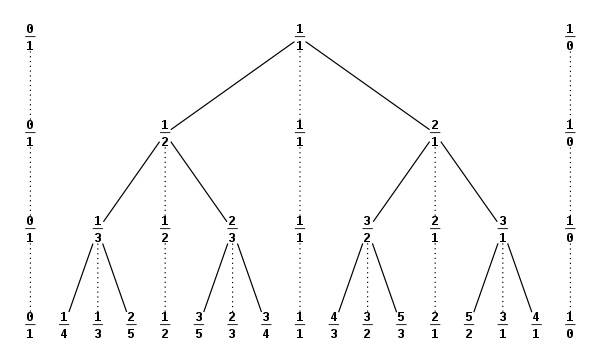
\includegraphics[scale=0.3]{figure2.png}

    序列里初始有两个元素$(0,1),(1,0)$,然后每次向序列相邻的两个元素$(x_1,y_1),(x_2,y_2)$中添加一个元素$(x_1+x_2,y_1+y_2)$,即可得到Stern–Brocot tree。
\end{definition}
\end{frame}

\begin{frame}{Stern–Brocot tree}

\begin{theorem}
	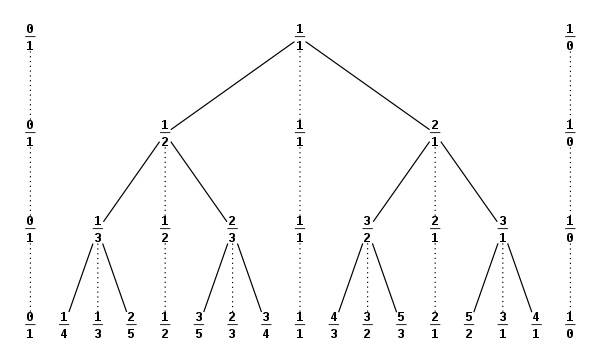
\includegraphics[scale=0.3]{figure2.png}

    对于树上相邻两点$(x_1,y_1),(x_2,y_2)$,有$|x_1y_2-x_2y_1|=1$。
\end{theorem}
\begin{proof}
    $|x_1(y_1+y_3)-(x_1+x_3)y_1|=|x_1y_3-x_3y_1|=1$。
    
    然后用数学归纳法。
\end{proof}
\end{frame}

\begin{frame}{Stern–Brocot tree}

\begin{theorem}
	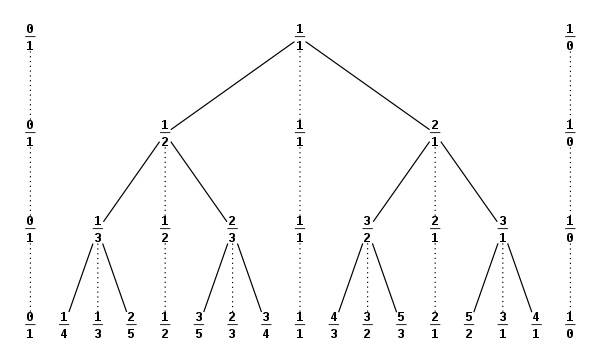
\includegraphics[scale=0.3]{figure2.png}

    若$|x_1y_2-x_2y_1|=1$,则$(x_1,y_1),(x_2,y_2)$在树上相邻。
\end{theorem}
\begin{proof}
    与上一个性质的证明类似。略。
\end{proof}
\end{frame}

\begin{frame}{Stern–Brocot tree}

\begin{theorem}
	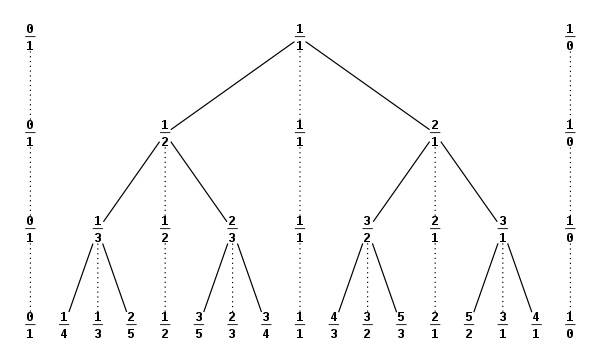
\includegraphics[scale=0.3]{figure2.png}

    设$(x,y)$是树上一点,则$\gcd(x,y)=1$。
\end{theorem}
\begin{proof}
    存在树上相邻一点$(u,w)$,使得$ux-wy=1$。
\end{proof}
\end{frame}

\begin{frame}{Stern–Brocot tree}

\begin{example}[accoders2169]
跳跳棋是在一条数轴上进行的。棋子只能摆在整点上。每个点不能摆超过一个棋子。我们用跳跳棋来做一个简单的游戏:棋盘上有$3$颗棋子, 分别在$a,b,c$这三个位置。我们要通过最少的跳动把他们的位置移动成$x,y,z$(棋子是没有区别的)。

跳动的规则很简单,任意选一颗棋子,对一颗中轴棋子跳动。跳动后两颗棋子距离不变。\textbf{一次只允许跳过$1$颗棋子}。

判断是否可以完成任务。如果可以,输出最少需要的跳动次数。

数据范围:棋子的坐标的绝对值不超过$10^9$。
\end{example}
\end{frame}

\begin{frame}{Stern–Brocot tree}

由于有一次只允许跳过$1$颗棋子的限制,所以两边往中间跳只有一种方案。而中间往两边跳有两种方案。

然后聪明的你可以发现,如果不考虑绝对坐标只考虑棋子之间的相对坐标差的话,这就是在Stern–Brocot tree上面跳。

所以如果有解,答案就是树上两个点的距离,用lca之类的不难求得。

当然这个题有绝对坐标必须相等的限制,所以还要判无解。我们就对他给的两个状态都疯狂地往父亲跳,在跳的过程中维护棋子的坐标,然后跳到根看看绝对坐标是否相等就可以了。注意往根跳的时候,可以发现这就是在做辗转相减,我们应该优化成辗转相除,不然会超时。

\end{frame}

\begin{frame}[plain]    %%谢谢
	\vspace{0.4\textheight}
	\begin{center}
		\Huge\color{blue}\bfseries Thanks!
	\end{center}
\end{frame}

\end{document}